\section{Đặc tả yêu cầu hệ thống}

\subsection{Yêu cầu chức năng}

Hệ thống thương mại điện tử thời trang được xây dựng nhằm hỗ trợ hoạt động mua sắm quần áo trực tuyến, đồng thời tích hợp công nghệ trí tuệ nhân tạo (AI) và thực tế tăng cường (Augmented Reality – AR) để nâng cao trải nghiệm người dùng. 

Hệ thống cho phép khách hàng tìm kiếm, lựa chọn và mua sản phẩm thời trang, thử quần áo ảo bằng AI Virtual Try-On, thử đồ thời gian thực bằng AR Try-On, đồng thời cung cấp chatbot AI hỗ trợ tư vấn sản phẩm và phối đồ. Ngoài ra, hệ thống còn hỗ trợ quản trị viên quản lý người dùng, sản phẩm, đơn hàng, nội dung và tài nguyên AI.

\textbf{a) Sơ đồ BFD}

Sơ đồ BFD mô tả các nhóm chức năng chính của hệ thống thương mại điện tử thời trang tích hợp AI và AR. Các chức năng được phân rã từ mức tổng quát đến các chức năng chi tiết nhằm thể hiện đầy đủ các nghiệp vụ của hệ thống.

\begin{figure}[H]
    \centering
    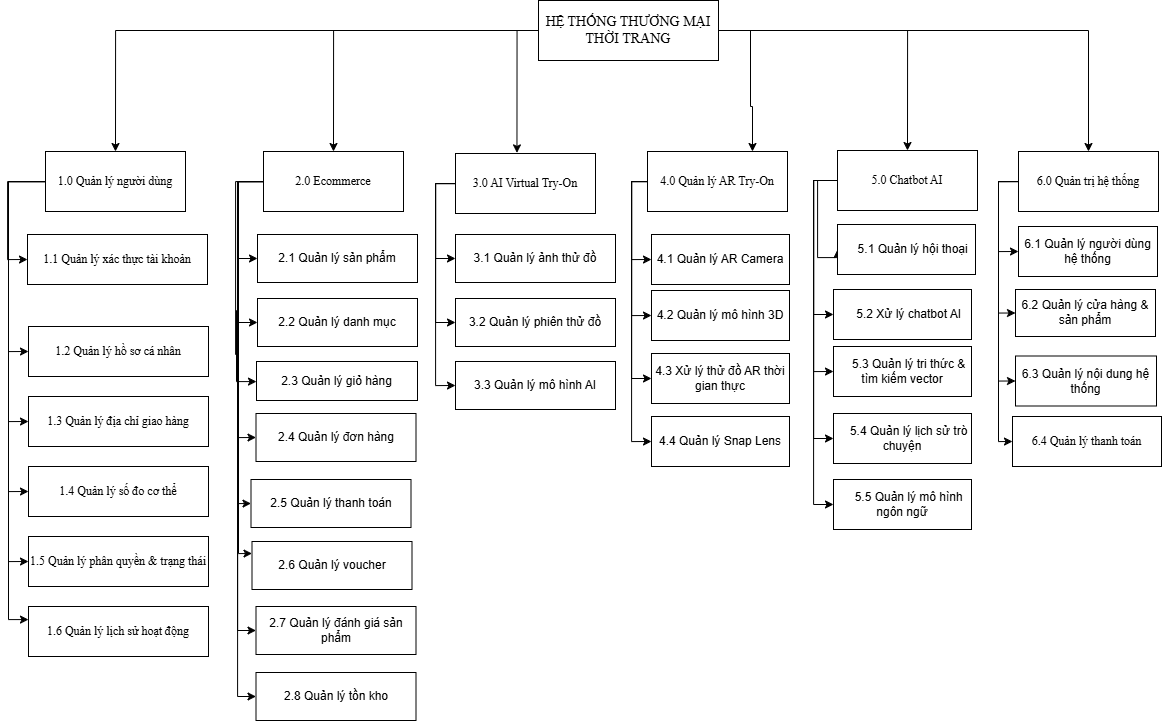
\includegraphics[width=\textwidth]{graphics/front/BFDtm.png}
    \caption{Sơ đồ BFD của hệ thống}
    \label{fig:bfd}
\end{figure}

\textbf{b) Mô tả ngắn gọn các nhóm chức năng}

\begin{itemize}

    \item \textbf{Quản lý người dùng}: 
    Cho phép người dùng đăng ký, đăng nhập bằng tài khoản hoặc Google, quản lý hồ sơ cá nhân, địa chỉ giao hàng, số đo cơ thể và lịch sử hoạt động trên hệ thống. Hệ thống cũng hỗ trợ phân quyền và quản lý trạng thái tài khoản.

    \item \textbf{Quản lý thương mại điện tử (Ecommerce)}: 
    Hỗ trợ quản lý sản phẩm, danh mục, giỏ hàng, đơn hàng, thanh toán trực tuyến, voucher giảm giá, đánh giá sản phẩm và quản lý tồn kho. Người dùng có thể tìm kiếm, lựa chọn và theo dõi trạng thái đơn hàng trực tuyến.

    \item \textbf{AI Virtual Try-On}: 
    Cho phép người dùng thử quần áo ảo bằng công nghệ AI thông qua việc tải ảnh người dùng và ảnh quần áo lên hệ thống. Hệ thống sử dụng mô hình FitDiT kết hợp xử lý keypoint và phân vùng cơ thể để sinh ảnh thử đồ ảo, đồng thời hỗ trợ đánh giá độ vừa vặn và gợi ý kích thước phù hợp.

    \item \textbf{Quản lý AR Try-On}: 
    Hỗ trợ thử quần áo theo thời gian thực bằng công nghệ thực tế tăng cường (AR). Hệ thống sử dụng Snap Camera Kit và mô hình 3D để hiển thị quần áo trực tiếp trên cơ thể người dùng thông qua camera.

    \item \textbf{Chatbot AI}: 
    Cung cấp chatbot AI hỗ trợ tư vấn thời trang, gợi ý sản phẩm và hỗ trợ khách hàng. Chatbot sử dụng mô hình ngôn ngữ lớn (LLM), kỹ thuật RAG và tìm kiếm vector để tạo phản hồi phù hợp theo ngữ cảnh hội thoại.

    \item \textbf{Quản trị hệ thống}: 
    Cho phép quản trị viên quản lý người dùng, cửa hàng, sản phẩm, nội dung hệ thống, tài nguyên AI và theo dõi thống kê doanh thu, hoạt động hệ thống cũng như hiệu năng xử lý AI.

\end{itemize}

\subsection{Yêu cầu phi chức năng}

Bên cạnh các yêu cầu chức năng, hệ thống cần đáp ứng các yêu cầu phi chức năng sau:

\begin{itemize}

    \item \textbf{Tính bảo mật}: 
    Hệ thống đảm bảo an toàn thông tin người dùng và dữ liệu hệ thống thông qua cơ chế xác thực JWT, Firebase Authentication và phân quyền truy cập theo vai trò người dùng.

    \item \textbf{Hiệu năng}: 
    Hệ thống có khả năng xử lý đồng thời nhiều yêu cầu truy cập. Các chức năng AI Virtual Try-On và AR Try-On cần đảm bảo thời gian phản hồi hợp lý và tối ưu tài nguyên GPU trong quá trình xử lý.

    \item \textbf{Tính khả dụng}: 
    Giao diện hệ thống thân thiện, dễ sử dụng trên nhiều thiết bị khác nhau. Các chức năng AR hoạt động trực tiếp trên trình duyệt mà không yêu cầu cài đặt thêm phần mềm.

    \item \textbf{Tính mở rộng}: 
    Hệ thống được thiết kế theo hướng module hóa, cho phép dễ dàng mở rộng thêm các chức năng AI, nâng cấp mô hình xử lý ảnh hoặc tích hợp thêm các công nghệ mới trong tương lai.

    \item \textbf{Độ tin cậy}: 
    Hệ thống hoạt động ổn định, đảm bảo dữ liệu không bị mất mát và duy trì khả năng phục hồi khi xảy ra lỗi trong quá trình xử lý.

    \item \textbf{Khả năng bảo trì}: 
    Mã nguồn được tổ chức rõ ràng theo kiến trúc frontend, backend và AI service riêng biệt nhằm hỗ trợ dễ dàng bảo trì, nâng cấp và triển khai hệ thống.

\end{itemize}